\appendix
\section{Extras}

\begin{frame}{Supplemental Slides}
 
 \begin{itemize}
  \item Discuss in depth topics should time allow
 \end{itemize}

\end{frame}

\begin{frame}{Propensity Score Issues}
 \begin{itemize}
  \item Unmeasured confounders
  \item Choice of pretreatment covariates in the propensity score model
  \item Different models and methods may lead to different conclusions
 \end{itemize}

\end{frame}

\begin{frame}{Joint Modelling (JM)}
 \begin{itemize}
  \item Assume ignorable MAR missing data mechanism
  \item Missing data imputed by sampling from a user specified distribution
  \item A lot of theory developed for Normal, not much else
  \begin{itemize}
   \item Normal imputation has been shown to perform well, even under non normality \cite{Demirtas2008}
  \end{itemize}
\item Idea: pull imputations by missing data row pattern
 \end{itemize}

\end{frame}

\begin{frame}{JM pseudocode}
 \begin{figure}[h!]
  \centering
    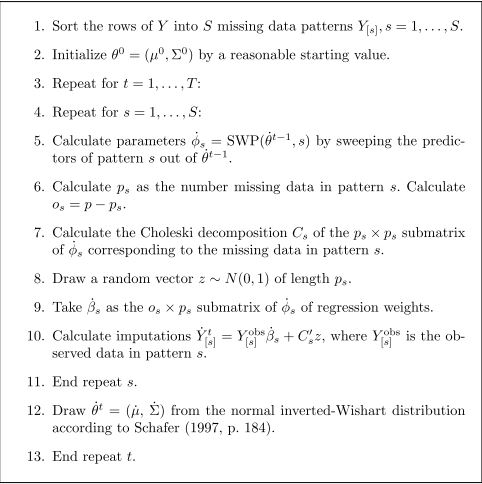
\includegraphics[width=0.6\textwidth]{jm_algo}
  \caption{Normal JM imputation pseudocode}
\label{fig:jmexample}
\end{figure}
%do I want to include the amelia algo?
\end{frame}

\begin{frame}{JM Pros and Cons}
Pros
 \begin{itemize}
  \item Fast
  \item Easy to derive posteriors with common distributions
 \end{itemize}

 Cons
 \begin{itemize}
  \item Inflexible
  \item Limited to known distributions
  \item How to deal with mixed categorical and continuous missing data
 \item Poor with derived variables
 \item Can give impossible combinations
 \end{itemize}

\end{frame}



\begin{frame}{Inference with Rubin's Rules}
 \begin{itemize}
  \item Assume that with complete data, inference on the estimand
  Q would be based on the statement $(Q- \hat{Q})\sim N(0,U)$
  \begin{itemize}
   \item $\hat{Q}$ is the statistic estimating Q
   \item $U$ is the variance-covariance of $(Q-\hat{Q})$
  \end{itemize}
   \item Since true T is not known, then
  $$\frac{Q-\hat{Q}}{\sqrt{T}}\sim t_{\nu}$$
  \item $\nu$ is given by \cite{Barnard1999}
  $$\nu=\frac{\nu_{old}\nu_{obs}}{\nu_{old}+\nu_{obs}}$$
\item Where $\nu_{obs}=\frac{\nu_{com}+1}{\nu_{com}+3}\nu_{com}(1-\frac{B + B/m}{T})$
\item $\nu_{com}$ is the hypothetical complete sample degrees of freedom
\item $\nu_{old}=\frac{m-1}{(\frac{B + B/m}{T})^2}$ 
 \end{itemize}

 \note{Requires normality
if not normal, transform}
\end{frame}

\begin{frame}{The Stack Method}
 \begin{itemize}
  \item Rubin's Rules work well, but not always
  \begin{itemize}
   \item Ex: partitioning the MI data on an imputed variable
   \item Taking the average is not a good idea
  \end{itemize}
    \item Solution: Stack the MI datasets on top of each other to get one huge dataset
    \begin{itemize}
     \item Will get unbiased results
     \item But sample size is falsely inflated, thus cannot trust variance
    \end{itemize}
 \end{itemize}
 \begin{figure}[h!]
  \centering
    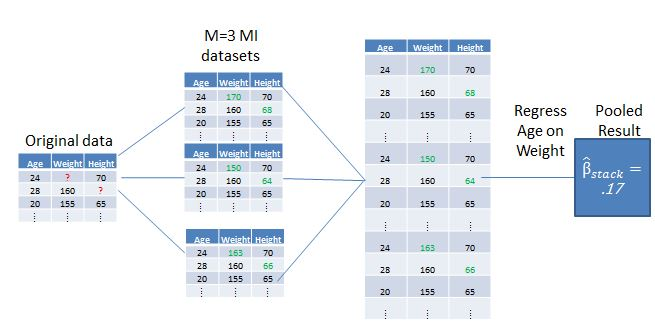
\includegraphics[width=0.6\textwidth]{stacked}
 % \caption{Normal JM imputation pseudocode}
\label{fig:stacked}
\end{figure}
\end{frame}

\begin{frame}{KM issues in the MI setting}
\begin{itemize}
\item Issue: Kaplan-Meier is not normally distributed
  \begin{itemize}
   \item Solution: Complimentary log-log transformation, pool \cite{Marshall2009}
  \end{itemize}
  \item Issue: Imputations leave one KM curve much shorter than the rest
  \begin{itemize}
   \item Solution 1: Truncate all curves at the lowest time
   \item Solution 2: Extend the curves out to the longest time
   \item Solution 3: Use the stacked method
  \end{itemize}

\end{itemize}
\end{frame}

\begin{frame}{Median Survival Time}
 \begin{itemize}
  \item Want a measure of central tendency
  \begin{itemize}
   \item Survival distributions often skewed, so mean is poor choice
  \end{itemize}
  \item Median: smallest time such that $\hat{S}(t)\leq .5$
\item Algorithm: Take MI Kaplan-Meier curve, observe first time it goes below 50\%
\item Confidence interval at median: the median of the upper and lower confidence bands
 \end{itemize}

\end{frame}

\begin{frame}{Log Rank Issues in MI setting}
\begin{itemize}
  \item Idea: Combine log rank tests from each MI dataset
  \begin{itemize}
  \item Problem: Wastes information and is unstable \cite{Marshall2009}
  \item Idea: Calculate log rank from the MI Kaplan-Meier curve
  \item Problem: Risk set and deaths no longer meaningful
  \end{itemize}
\end{itemize}
\end{frame}

\begin{frame}{Setting up the model- Issues}
\begin{itemize}
 \item Many categorical variables 
 \item Collinearity between predictors
 \item Variables with poor influx/outflux \cite{VanBuuren2012}
 \item How many iterations and imputations to draw?
\end{itemize}

\end{frame}


\begin{frame}{Validity Checks}
\begin{figure}[h!]
  \centering
 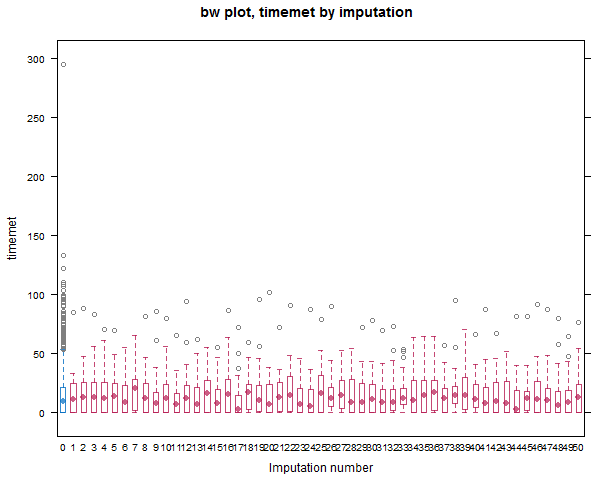
\includegraphics[width=.5\textwidth]{bw_timemet}%
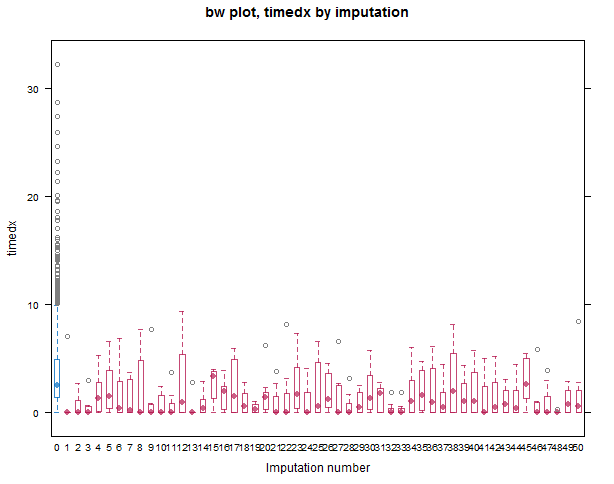
\includegraphics[width=.5\textwidth]{bw_timedx} 
\label{fig:bwcheck}
\caption{BW plot checks}
\end{figure}
\end{frame}

\begin{frame}{Tabular Checks}
 \begin{figure}[h!]
  \centering
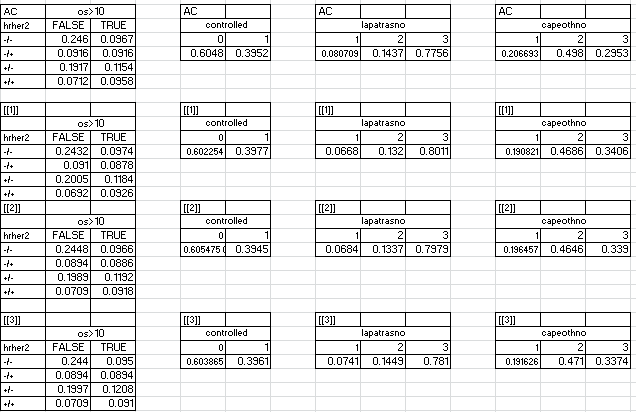
\includegraphics[width=.8\textwidth]{tabchecks} 
  \caption{Selected tabluar checks}
\label{fig:tabcheck}
\end{figure}

\end{frame}




\begin{frame}{Base model}
 \begin{table}[]
\centering
\adjustbox{max height=\dimexpr\textheight-5.5cm\relax,
           max width=\textwidth}{
\begin{tabular}{|c|c|c|c|c|c|c|c|c|}
\hline
                                                       &                                  &      & \begin{tabular}[c]{@{}c@{}}AC \\ n= 845\end{tabular} &                 &  &      & MI                                                 &                                                            \\ \hline
Variable                                               & Contrast                         & HR   & \begin{tabular}[c]{@{}c@{}}95\% \\ CI\end{tabular}   & pvalue          &  & HR   & \begin{tabular}[c]{@{}c@{}}95\% \\ CI\end{tabular} & \begin{tabular}[c]{@{}c@{}}pvalue\\  (t test)\end{tabular} \\ \hline
HR/HER2                                                & -/+ vs. -/-                      & 0.57 & (0.46,0.71)                                          & \textless0.0001 &  & 0.59 & (0.48,0.72)                                        & \textless0.0001                                            \\ \hline
                                                       & +/- vs. -/-                      & 0.66 & (0.54,0.81)                                          & \textless0.0001 &  & 0.63 & (0.52,0.76)                                        & \textless0.0001                                            \\ \hline
                                                       & +/+ vs. -/-                      & 0.4  & (0.31,0.50)                                          & \textless0.0001 &  & 0.4  & (0.32,0.50)                                        & \textless0.0001                                            \\ \hline
Age                                                    & \textgreater 60 vs. \textless 60 & 1.37 & (1.13,1.65)                                          & 0.0011          &  & 1.45 & (1.22,1.72)                                        & \textless0.0001                                            \\ \hline
Dx to BM                                               & \textgreater 6 vs. \textless 6   & 0.66 & (0.54,0.82)                                          & 0.00013         &  & 0.71 & (0.59,0.86)                                        & 0.0002                                                     \\ \hline
First DM                                               & Brain vs. Oth                    & 0.8  & (0.66,0.97)                                          & 0.026           &  & 0.83 & (0.70,0.99)                                        & 0.02                                                       \\ \hline
Race                                                   & Hisp. Vs. White                  & 0.85 & (0.68,1.07)                                          & 0.17            &  & 0.88 & (0.71,1.08)                                        & 0.11                                                       \\ \hline
                                                       & Black vs. White                  & 1.31 & (1.06,1.63)                                          & 0.014           &  & 1.25 & (1.02,1.52)                                        & 0.015                                                      \\ \hline
                                                       & Other vs. White                  & 0.65 & (0.40,1.04)                                          & 0.075           &  & 0.7  & (0.45,1.07)                                        & 0.05                                                       \\ \hline
\begin{tabular}[c]{@{}c@{}}\# prior \\ Rx\end{tabular} & \textgreater2 vs. 0-2            & 1.58 & (1.31,1.91)                                          & \textless0.0001 &  & 1.53 & (1.29,1.82)                                        & \textless0.0001                                            \\ \hline
BM type                                                & Mult. Vs. Single                 & 1.45 & (1.20,1.76)                                          & \textless0.0001 &  & 1.48 & (1.24,1.76)                                        & \textless0.0001                                            \\ \hline
                                                       & LMD vs. Single                   & 1.6  & (1.21,2.13)                                          & 0.001           &  & 1.58 & (1.25,2.00)                                        & \textless0.0001                                            \\ \hline
Sys. Cont.                                             & Yes vs. No                       & 0.71 & (0.61,0.83)                                          & \textless0.0001 &  & 0.73 & (0.63,0.85)                                        & \textless0.0001                                            \\ \hline
\end{tabular}
}
\caption{AC and MI baseline Cox regression}
\label{fig:acmicox}
\end{table}

\end{frame}



\begin{frame}{Issues with Propensity Score in our Setting}
\begin{itemize}
 \item Problem: Theory was developed for binary treatments, we have ternary
 \begin{itemize}
  \item Solution: Run each treatment as binary, then compare groups
 \end{itemize}
\item Propensity score model specification
\begin{itemize}
 \item Solution: Boosting, subject to KS statistic minimization
\end{itemize}
\end{itemize}
 
\end{frame}

\begin{frame}{Propensity Score Box and Whisker Checks}
 \begin{figure}[h!]
  \centering
  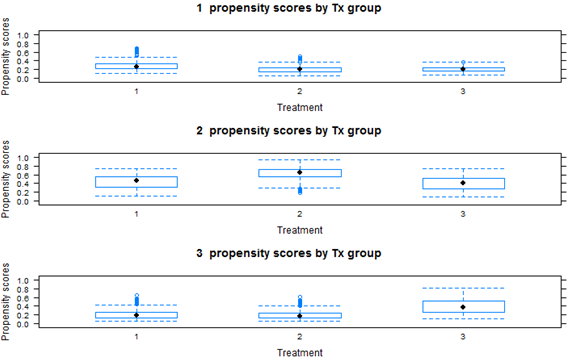
\includegraphics[width=.5\textwidth]{ps_histo1}%
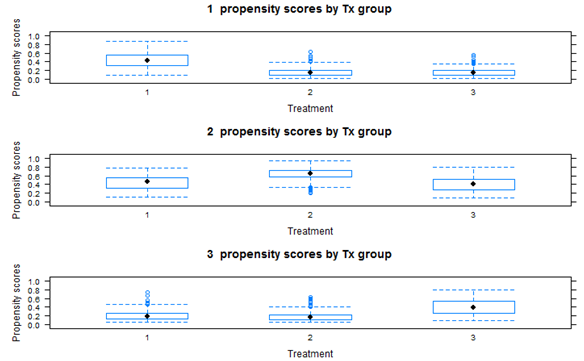
\includegraphics[width=.5\textwidth]{ps_histo2} 
  \caption{Selected PS BW plots}
\label{fig:psbw}
\end{figure}
\end{frame}


%put boosting algo here if I have time
\begin{frame}{Boosting}
 
  \begin{figure}[h!]
  \centering
 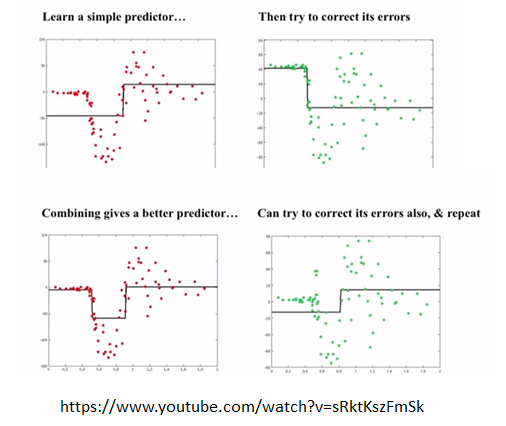
\includegraphics[width=.8\textwidth]{boosting}
  \caption{Boosting Algorithm}
\label{fig:boosting}
\end{figure}
\end{frame}
